% Kapitel 9 - Fazit
\section{Implementation}
In chapter \ref{sec:Algorithm definition}, a comprehensive and exhaustive study of different approaches to compression algorithm was conducted. The conclusion drawn was that an approach with mathematical reduction with a combination of data filtering was the most suitable for the type of data-sets being dealt with in this thesis, i.e .asc files. In this chapter, the implementation of the conclusion from previous chapter would be discussed.

\subsection{Algorithm Selection}
As per figure \ref{fig:Weighted Analysis}, real time processing via mathematical reduction is the most suitable method to achieve optimal fulfillment of the requirements. The implementation of this method requires to easy access to :

\begin{itemize}
    \item Test systems with CANoe pre-installed
    \item CAPL coding environment
    \item Data files for testing and validation
\end{itemize}

CANoe is a licensed tool provided by Vector Informatik GmbH. It is a complex and large tool to use with numerous features suitable for different types of uses in diversified environments in the domain of verification \& validation. The licenses are extremely expensive and hence the easy access to such tools is also restricted. Usually such licenses are purchased in limited quantities and shared in team pools for various projects and hence the access is always determined by priority of implementation basis. 

Vector provides three types of licensing for CANoe tool, each of which have their own utilities and limitations. The three types of licenses are :

\begin{itemize}
    \item CANoe pro
    \item CANoe run
    \item CANoe pex
\end{itemize}

The pro version is the highest tier license version of CANoe. As the name suggests, the license gives access to all features of CANoe tool which also includes CAPL coding environment. The run license provides limited access to CANoe environment where it is possible to run and analyse all the pre-existing test setups and programs. The user is restricted from changing any configurations in the setups using run license. The pex license is the basic license required to view CANoe tool. It is useful for viewing the tool and it's setup and configurations, however, creating, running or changing configurations and setups are prohibited. Here, \ref{fig:CANoe Licenses}, one can see the features included with pro license.

\begin{figure}[h]
    	\centering
    	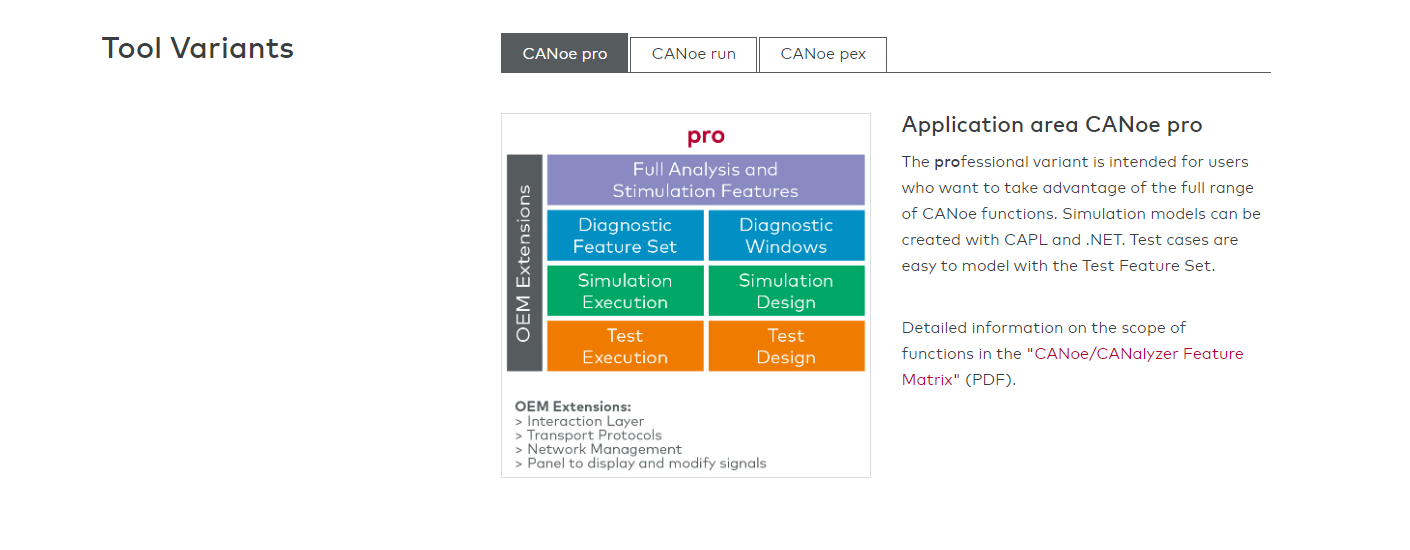
\includegraphics[width= 1\textwidth]{images/CANoe license type.png}
    	\caption [Licenses]{CANoe licenses}  
    	\label{fig:CANoe Licenses}
\end{figure}

\begin{figure}[h]
    	\centering
    	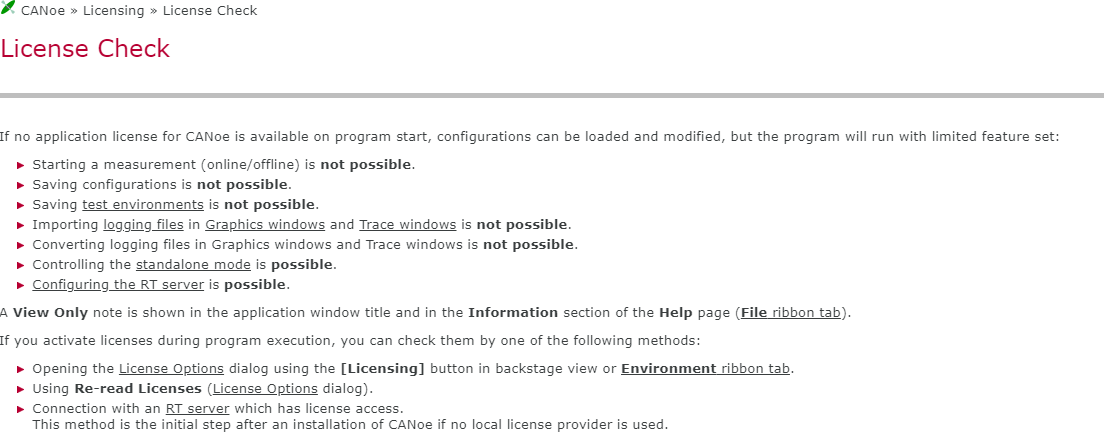
\includegraphics[width= 1\textwidth]{images/CANoe license restrictions.png}
    	\caption [Restrictions]{CANoe restrictions}  
    	\label{fig:CANoe Restrictions}
\end{figure}


\clearpage

Figure \ref{fig:CANoe Restrictions} shows the restrictions involved with limited access licenses. Hence, it is of utmost importance to have access to the pro version of licenses. At CES, CANoe pro licenses are available to use for test systems. However, it is subjected to availability of the test systems. Since, multiple projects require the availability of test systems, getting a free-to-use access to test systems is difficult. Since, implementing the algorithm requires constant access to development environment for development, testing and validation an alternative was required to overcome the limited access to the test systems. 

As discussed in the conclusion of \ref{sec:Algorithm definition}, the weighted analysis revealed two possible alternatives for implementation of mathematical reduction based compression algorithm : \\
1) Real Time Processing    2) Batch Processing or Post-Processing 

Since, the approach for compressing data and reducing data size in both processes is identical, the use of an alternative to the real time processing approach can be considered and tested to verify if the desired compression is achieved or not. Once, the data compression is verified and validated, the algorithm can be transferred from post-processing to real-time processing with necessary changes. This will be discussed as part of scope of development for future.

To conclude, the compression algorithm with post processing will be used as the base for implementation study and the development platform to be used for this purpose will be python.

But before moving to development phase, it is necessary to define the structure of the program. Without a proper structure, it is easy to lose the sight of goal or worse get entangled in unproductive development hassles irrelevant to the goals. Designing the structure of a program before starting to code is an important step in the software development process. It can help ensure that the code is well-organized, maintainable, and easy to understand. Here are some common ways to design the structure of a program: 

\begin{itemize}
    \item Pseudocode: Pseudocode is a high-level, human-readable description of the steps a program should take to solve a problem. It is written in a syntax that resembles a programming language but is not meant to be executed. Pseudocode can be a useful tool for designing the structure of a program, as it allows you to think through the problem and get a rough idea of the steps your code will need to take before writing any actual code.
    \item Flowcharts: Flowcharts are diagrams that show the flow of control through a program. They can be used to represent the structure of a program, making it easy to see the different parts of the program and how they relate to each other. Flowcharts can be a helpful tool for designing complex programs, as they make it easy to see the logic of the program at a high level.
    \item Mind maps: Mind maps are diagrams that show the relationships between different ideas or concepts. They can be used to design the structure of a program by breaking the problem down into smaller parts and showing how they fit together. Mind maps can be a good way to get a bird's eye view of the program and see how all of the pieces fit together.
    \item Diagrams and schematics: You can also use other types of diagrams and schematics to design the structure of a program. For example, you might use a block diagram to show the relationships between different parts of the program, or a state diagram to show the different states that a program can be in and the transitions between those states.
    \item Code sketching: Finally, you can also start designing the structure of a program by sketching out some of the code on paper. This can be a good way to experiment with different approaches and see what code structures make the most sense for the problem you are trying to solve.
\end{itemize}

\newpage
\subsection{Initial Setup}

Python is a high-level, interpreted, general-purpose programming language. It was first released in 1991 by Guido van Rossum and has since become one of the most widely used programming languages in the world.

Python is popular for its simple, easy-to-read syntax which allows developers to express concepts in fewer lines of code compared to other programming languages. It is also highly versatile and can be used for a variety of applications, including web development, scientific computing, data analysis, artificial intelligence, and more. One of the main benefits of using Python is its extensive library of modules and packages, which makes it easy to perform common programming tasks without having to write extensive amounts of code. This has led to a large and active community of developers who continuously contribute to the development and improvement of the language.

There are currently two stable versions of Python in widespread use: Python 2 and Python 3. Python 2 was first released in 2000, and although it is still in use, its development has been largely discontinued in favor of Python 3. Python 3 was first released in 2008 and has since become the standard version of Python, with many improvements over Python 2. The compression algorithm discussed in this thesis has thus been designed exclusively using Python 3. 

Python programs can be written and executed by means of a terminal or IDE also known as Integrated development environment. The scripts, or codes, are written and saved with a ".py" extension. An IDE was selected and utilized for the purpose of development of compression algorithm in this thesis. An integrated development environment (IDE) is a software application that provides comprehensive facilities to computer programmers for software development. An IDE normally consists of at least a source code editor, build automation tools and a debugger \cite{PyWiki}. IDEs maximize user productivity by providing easy access to multiple components of the coding environment such as code alignment, errors \& warnings indicators, easy install of packages library etc.   

One aim of the IDE is to reduce the configuration necessary to piece together multiple development utilities. Instead, it provides the same set of capabilities as one cohesive unit. Reducing setup time can increase developer productivity, especially in cases where learning to use the IDE is faster than manually integrating and learning all of the individual tools. Tighter integration of all development tasks has the potential to improve overall productivity beyond just helping with setup tasks. For example, code can be continuously parsed while it is being edited, providing instant feedback when syntax errors are introduced, thus allowing developers to debug code much faster and more easily with an IDE.

Some IDEs are dedicated to a specific programming language, allowing a feature set that most closely matches the programming paradigms of the language.\cite{PyWiki} PyCharm is one such IDE dedicated for the development of python based programs. It provides code analysis, a graphical debugger, an integrated unit tester, integration with version control systems, and supports web development with Django. It is cross-platform, working on Microsoft Windows, macOS and Linux. PyCharm has two editions : Professional and Community. PyCharm Community Edition is less extensive than the Professional Edition. While PyCharm professional is suited for both scientific and web python development with HTML, JS and SQL support at a subscription price, PyCharm Community edition is a free version for pure python development aimed at hobbyist or beginners who want to develop programs without integration to web. For the purpose of this thesis, the PyCharm Community Edition is used since web based development is not involved here. Below is a representation of the PyCharm IDE interface:

\begin{figure}[h]
    	\centering
    	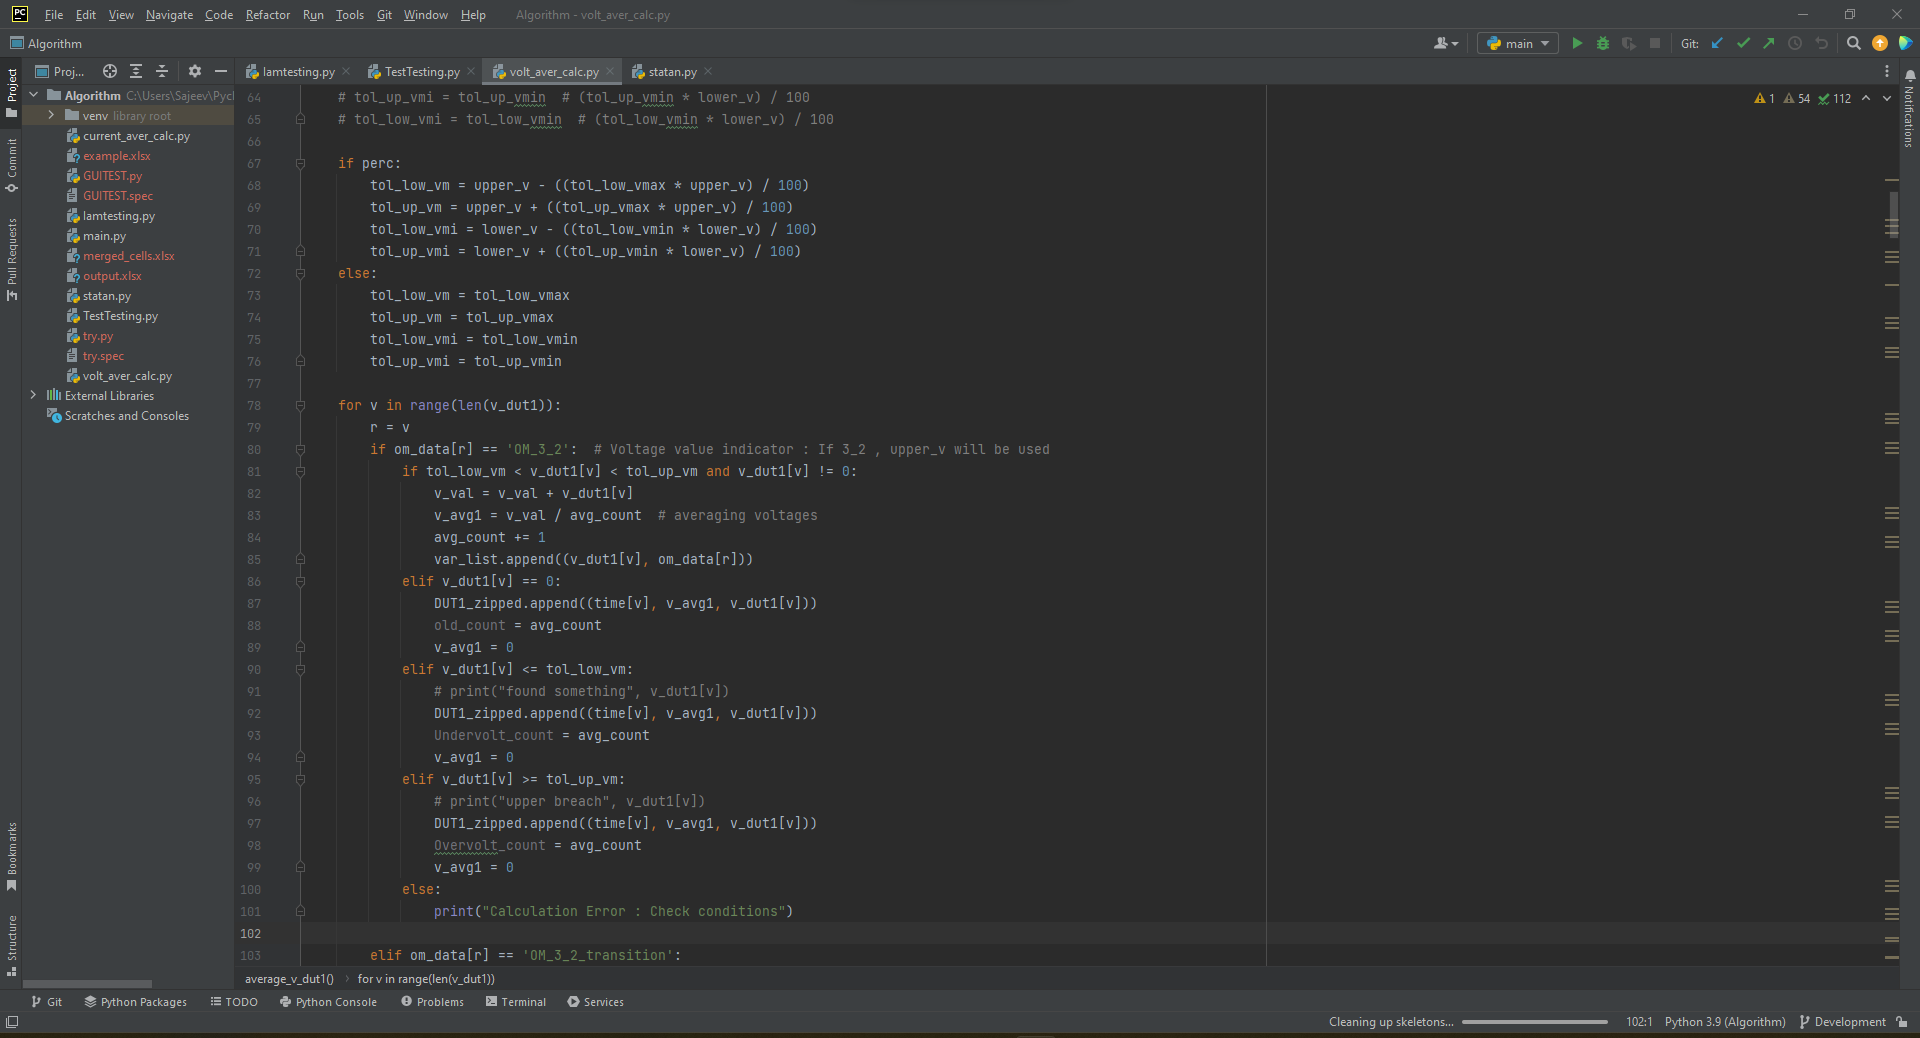
\includegraphics[width= 1\textwidth]{images/pycharm.png}
    	\caption [PyCharm]{PyCharm Interface}  
    	\label{fig:Pycharm interface}
\end{figure}



\newpage
    
\subsection{Einschränkungen}


\paragraph{Evaluation} 
Bla bla.

\paragraph{Konzept}


%\input{chap9x} %chap9_futurework_limitations}